\chapter{Dinámica del citoesqueleto y motilidad celular}\label{ch:b3:cytoskeleton-motility}

Un neutrófilo que persigue a una bacteria por un tejido repta a diez
micrómetros por minuto y cambia de rumbo en segundos cuando el rastro se
desplaza. Una vesícula de neurotransmisor fabricada en el cuerpo celular
de una motoneurona recorre un metro por el axón hasta el pie, arrastrada
por una proteína motora que da pasos de ocho nanómetros, cien por
segundo, durante quince días. Los \omterm{def:b3:cytoskeleton-motility:cilia}{cilios} que tapizan la tráquea baten
doce veces por segundo en ondas coordinadas que llevan hasta la garganta
el polvo inhalado de un día. Todo esto lo hacen tres clases de filamento
proteico que se ensamblan y se desensamblan en segundos, y unos motores
que queman una molécula de ATP por paso. El citoesqueleto no es en
absoluto un esqueleto en el sentido de un armazón fijo; es un conjunto de
polímeros en recambio constante, cuya dinámica \emph{es} el mecanismo de
la forma, la división y el movimiento. Este capítulo trata de los
polímeros y su cinética, de los motores y la física que los limita, del
reptar de una célula y del batido de \omterm{def:b3:cytoskeleton-motility:cilia}{cilios} y flagelos.

\section{Tres polímeros}

\begin{definition}[Filamentos de actina, microtúbulos, filamentos intermedios]\label{def:b3:cytoskeleton-motility:filaments}
\index{filamento de actina}\index{microtúbulo}\index{filamento intermedio}\index{polaridad!de los filamentos}\index{centrosoma}
Un \emph{filamento de actina} es un polímero helicoidal de dos hebras de
actina globular, de \qty{7}{nm} de grosor, con cada subunidad ocupando
\qty{2.7}{nm} a lo largo del eje, y es polar: el extremo \emph{barbado}
(más) crece más deprisa que el extremo \emph{puntiagudo} (menos), y cada
subunidad lleva un ATP que se hidroliza tras la incorporación. Un
\emph{microtúbulo} es un tubo hueco de \qty{25}{nm} de diámetro externo
construido con trece protofilamentos de dímeros de
$\alpha\beta$-tubulina (\qty{8}{nm} por dímero), también polar, con su
extremo \emph{más} creciendo más deprisa y su extremo \emph{menos} anclado
por lo común en el \emph{centrosoma}, cerca del núcleo; la subunidad
$\beta$ hidroliza su GTP tras la incorporación. Un \emph{filamento
intermedio} es una cuerda de \qty{10}{nm} hecha de proteínas en hélice
enrollada (queratinas en los epitelios, vimentina en el mesénquima,
neurofilamentos en los axones, laminas bajo la envoltura nuclear),
apolar, sin nucleótido y mucho más estable --- un cable que soporta
tensión más que una vía dinámica. La actina se sitúa sobre todo bajo la
membrana plasmática y en las protrusiones; los microtúbulos irradian
desde el centrosoma y sirven de vías del transporte a larga distancia y
de huso; y los filamentos intermedios dan a la célula y a su núcleo su
resistencia mecánica.
\end{definition}

\begin{omfigure}
\begin{tikzpicture}[every node/.style={font=\scriptsize}, >=stealth]
  % actin
  \begin{scope}
    \foreach \i in {0,...,11} { \fill[omThm!70] ({\i*0.4},{0.12*sin(\i*60)}) circle (0.17); }
    \node[below, align=center] at (2.2,-0.5) {filamento de actina, \qty{7}{nm}\\hélice de dos hebras, actina-ATP\\subunidad de \qty{2.7}{nm} a lo largo del eje};
    \node[left] at (-0.3,0) {$-$ puntiagudo}; \node[right] at (4.6,0) {barbado $+$};
  \end{scope}
  % microtubule
  \begin{scope}[xshift=7.2cm]
    \draw[thick, fill=omDef!25] (0,-0.55) rectangle (4.4,0.55);
    \foreach \y in {-0.35,-0.15,0.05,0.25} \draw[omDef] (0,\y) -- (4.4,\y);
    \foreach \x in {0.4,0.8,...,4.0} \draw[omDef] (\x,-0.55) -- (\x,0.55);
    \draw[thick] (4.4,0) ellipse (0.18 and 0.55); \draw[thick, fill=white] (4.4,0) ellipse (0.09 and 0.38);
    \node[below, align=center] at (2.2,-0.65) {microtúbulo, \qty{25}{nm}\\13 protofilamentos de $\alpha\beta$-tubulina (GTP)\\dímero de \qty{8}{nm} de largo};
    \node[left] at (-0.2,0) {$-$}; \node[right] at (4.7,0) {$+$};
  \end{scope}
  % intermediate filament
  \begin{scope}[yshift=-2.9cm, xshift=3.6cm]
    \foreach \dd in {-0.12,0,0.12} \draw[omMeth!70!black, thick] plot[domain=0:4.4, samples=60] (\x, {\dd + 0.1*sin(\x*200 + \dd*400)});
    \node[below, align=center] at (2.2,-0.4) {filamento intermedio, \qty{10}{nm}\\cuerda en hélice enrollada (queratina, vimentina, lamina), sin polaridad ni nucleótido};
  \end{scope}
\end{tikzpicture}

{\small Los tres filamentos, a escala en diámetro. Los polímeros de
actina y de tubulina son polares e hidrolizan un nucleótido tras el
ensamblaje, que es lo que los hace dinámicos; el \omterm{def:b3:cytoskeleton-motility:filaments}{filamento intermedio} es
una cuerda apolar construida para durar.}
\end{omfigure}

\begin{omfigure}
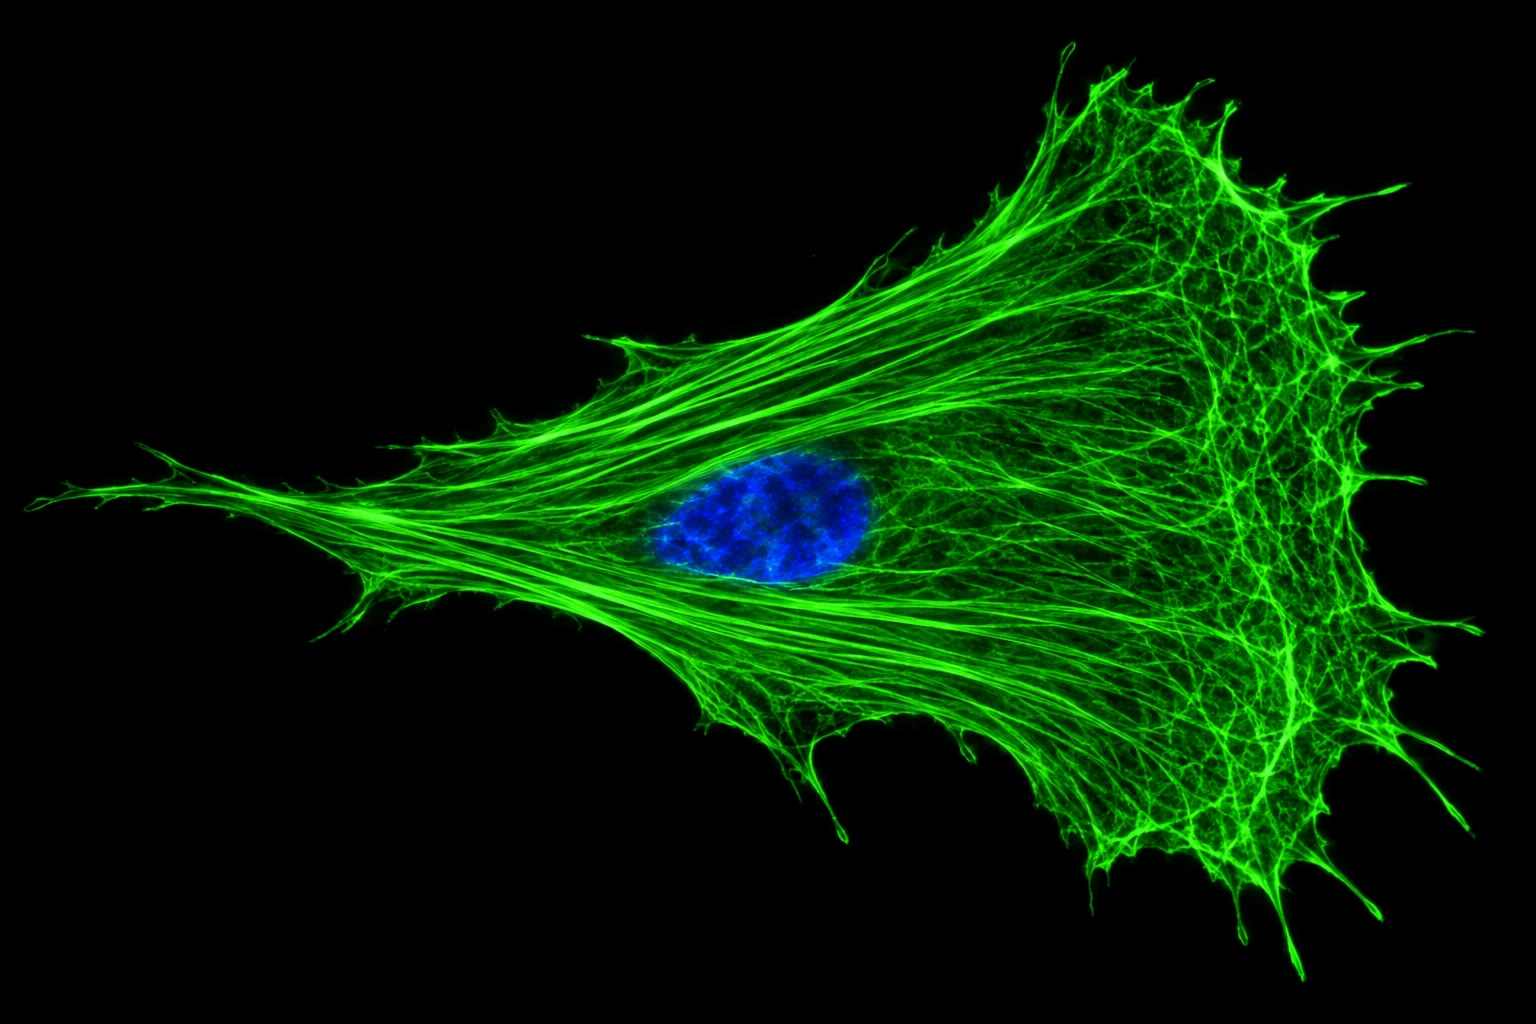
\includegraphics[width=0.54\linewidth]{images/book5/ai/b5-09-fibroblast-actin.jpg}\hspace{0.03\linewidth}
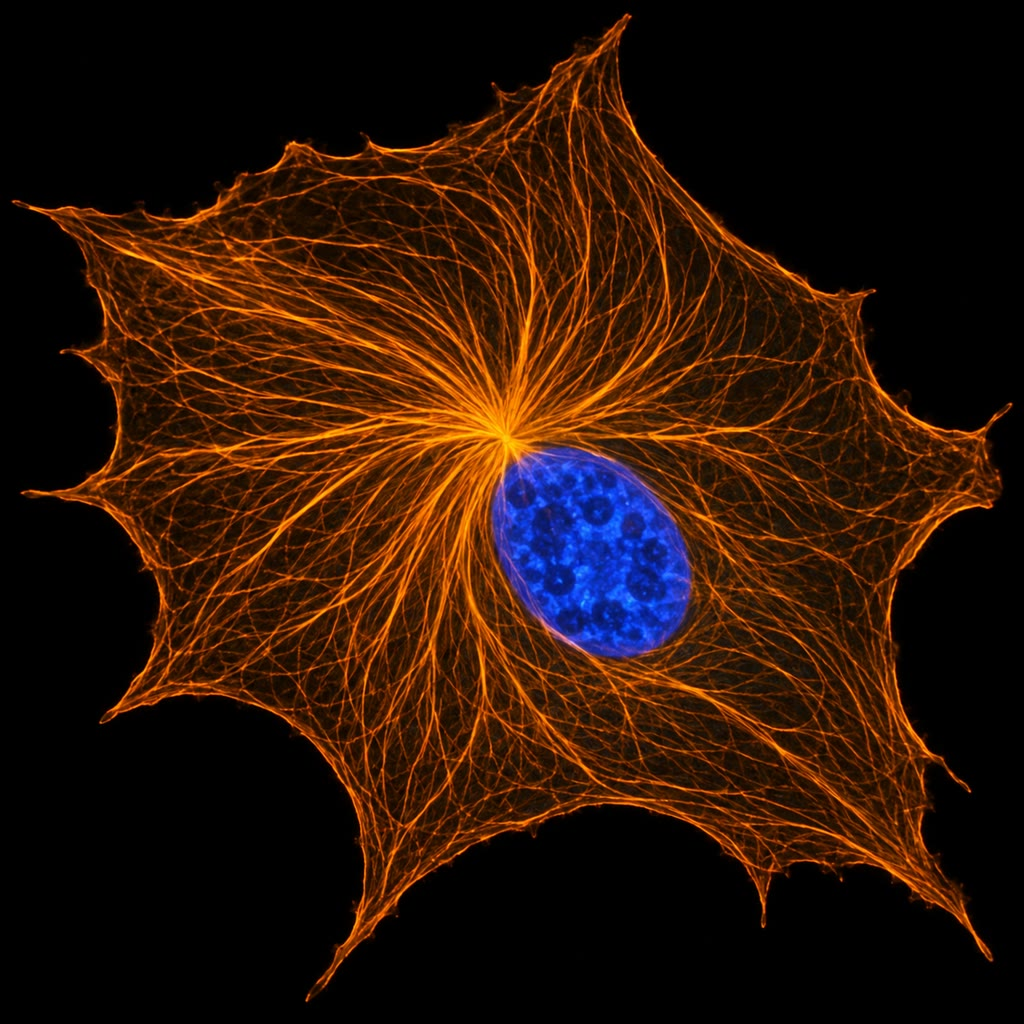
\includegraphics[width=0.36\linewidth]{images/book5/ai/b5-09-microtubules.jpg}

{\small Izquierda: actina (verde) en un fibroblasto que migra ---
fibras de tensión que cruzan el cuerpo y una malla densa en el amplio
borde delantero de la derecha. Derecha: \omterm{def:b3:cytoskeleton-motility:filaments}{microtúbulos} (naranja) que
irradian desde el \omterm{def:b3:cytoskeleton-motility:filaments}{centrosoma}, junto al núcleo (azul), hasta el margen de
la célula.}
\end{omfigure}

\section{La cinética de un polímero}

\begin{theorem}[Concentración crítica y noria de subunidades]\label{thm:b3:cytoskeleton-motility:treadmilling}
\index{concentración crítica}\index{noria de subunidades}
Supóngase que un extremo de un filamento añade subunidades a velocidad
$k_{\text{on}}C$, con $C$ la concentración de monómero libre, y las
pierde a velocidad $k_{\text{off}}$. El extremo crece si $C$ supera su
\emph{\omterm{thm:b3:cytoskeleton-motility:treadmilling}{concentración crítica}} $C_{c} = k_{\text{off}}/k_{\text{on}}$ y se
encoge por debajo de ella. Si los dos extremos tienen concentraciones
críticas distintas, $C_{c}^{+}
< C_{c}^{-}$, entonces en el estado estacionario en el que el filamento
ni se alarga ni se acorta la concentración de monómero es
\[
C_{\text{ss}} = \frac{k_{\text{off}}^{+} + k_{\text{off}}^{-}}
{k_{\text{on}}^{+} + k_{\text{on}}^{-}},
\qquad C_{c}^{+} < C_{\text{ss}} < C_{c}^{-},
\]
y el extremo más crece mientras el extremo menos se encoge al mismo
ritmo $J = k_{\text{on}}^{+}C_{\text{ss}} - k_{\text{off}}^{+} > 0$: las
subunidades fluyen por el filamento de más a menos --- la \emph{\omterm{thm:b3:cytoskeleton-motility:treadmilling}{noria de
subunidades}} --- al precio de un nucleótido hidrolizado por subunidad.
\end{theorem}
\begin{proof}
La velocidad neta en un extremo es $k_{\text{on}}C - k_{\text{off}}$,
nula en $C_{c}$. Que la longitud sea constante exige que la suma de las
dos velocidades netas se anule, lo que da $C_{\text{ss}}$; está entre las
dos concentraciones críticas porque es una media ponderada de ellas
($C_{\text{ss}} =
(k_{\text{on}}^{+}C_{c}^{+} + k_{\text{on}}^{-}C_{c}^{-})/(k_{\text{on}}^{+}
+ k_{\text{on}}^{-})$). Por encima de $C_{c}^{+}$ el extremo más crece;
por debajo de $C_{c}^{-}$ el extremo menos se encoge; y el flujo es la
velocidad neta del extremo más. Dos extremos del mismo polímero químico
tendrían el mismo $C_{c}$ (la misma constante de equilibrio), de modo que
una diferencia exige que la subunidad cambie tras incorporarse --- la
hidrólisis de ATP o de GTP ---, lo que hace que los extremos difieran y
paga el flujo.
\end{proof}

\begin{example}[La actina en el tubo de ensayo]\label{ex:b3:cytoskeleton-motility:actin-numbers}
Para la actina-ATP, $k_{\text{on}}^{+} = \qty{11.6}{\micro M^{-1}.s^{-1}}$
y $k_{\text{off}}^{+} = \qty{1.4}{s^{-1}}$ ($C_{c}^{+} = \qty{0.12}{\micro
M}$); $k_{\text{on}}^{-} = \qty{1.3}{\micro M^{-1}.s^{-1}}$ y
$k_{\text{off}}^{-} = \qty{0.8}{s^{-1}}$ ($C_{c}^{-} = \qty{0.6}{\micro
M}$). Entonces $C_{\text{ss}} = 2.2/12.9 = \qty{0.17}{\micro M}$ y $J =
11.6\times 0.17 - 1.4 = 0.6$ subunidades por segundo: \qty{1.6}{nm/s},
imperceptible. En una célula los filamentos giran cien veces más deprisa,
porque la cofilina corta y despoja de la vieja actina-ADP los extremos
puntiagudos, la profilina carga actina-ATP fresca en los extremos
barbados y las proteínas de caperuza deciden qué extremos barbados pueden
crecer siquiera: el polímero desnudo aporta el mecanismo y los reguladores
aportan la velocidad.
\end{example}

\begin{omfigure}
\begin{tikzpicture}
\begin{axis}[
  width=0.7\linewidth, height=5.6cm,
  axis x line=bottom, axis y line=left,
  xmin=0, xmax=1.0, ymin=-1.6, ymax=4,
  xlabel={actina libre ($\unit{\micro M}$)}, ylabel={velocidad neta (subunidades/s)},
  xlabel style={font=\small, at={(axis description cs:0.5,-0.12)}, anchor=north},
  ylabel style={font=\small},
  tick label style={font=\small}, xtick={0,0.2,0.4,0.6,0.8,1.0}, ytick={-1,0,1,2,3,4},
  clip=false,
]
\addplot[thin, gray, domain=0:1.0, samples=2] {0};
\addplot[very thick, omThm, domain=0:0.46, samples=2] {11.6*x-1.4};
\addplot[very thick, omDef, domain=0:1.0, samples=2] {1.3*x-0.8};
\draw[dashed, gray] (axis cs:0.17,-1.6) -- (axis cs:0.17,4);
\node[font=\scriptsize, omThm, anchor=south east] at (axis cs:0.44,3.1) {extremo barbado};
\node[font=\scriptsize, omDef, anchor=north west] at (axis cs:0.62,-0.25) {extremo puntiagudo};
\node[font=\scriptsize, anchor=south west] at (axis cs:0.19,3.5) {$C_{\text{ss}}$};
\fill[omThm] (axis cs:0.12,0) circle (2pt); \node[font=\scriptsize, anchor=north east] at (axis cs:0.11,-0.05) {$C_{c}^{+}$};
\fill[omDef] (axis cs:0.6,0) circle (2pt); \node[font=\scriptsize, anchor=south west] at (axis cs:0.61,0.05) {$C_{c}^{-}$};
\end{axis}
\end{tikzpicture}

{\small Velocidad neta de crecimiento de cada extremo de un \omterm{def:b3:cytoskeleton-motility:filaments}{filamento de
actina} frente al monómero libre, con las constantes del ejemplo. Entre
las dos concentraciones críticas el extremo barbado crece y el
puntiagudo se encoge; en la línea discontinua ambas se cancelan
exactamente y el filamento funciona como una noria.}
\end{omfigure}

\begin{definition}[Inestabilidad dinámica]\label{def:b3:cytoskeleton-motility:instability}
\index{inestabilidad dinámica}\index{caperuza de GTP}\index{catástrofe}
Los \omterm{def:b3:cytoskeleton-motility:filaments}{microtúbulos} hacen algo más extraño que la noria. Un extremo más en
crecimiento lleva una \emph{caperuza de GTP} de dímeros recién añadidos;
por detrás de ella el GTP se hidroliza, y la tubulina-GDP, que prefiere
una conformación curvada, se mantiene recta en la red bajo tensión. Si se
pierde la caperuza --- el extremo se detiene, o el crecimiento se frena
---, los protofilamentos tensados se despegan hacia fuera y el
\omterm{def:b3:cytoskeleton-motility:filaments}{microtúbulo} se acorta a \qty{300}{nm/s}, veinte veces su velocidad de
crecimiento: una \emph{catástrofe}, que termina cuando un dímero con GTP
se posa y se forma una caperuza nueva (un \emph{rescate}). En una misma
población, por tanto, unos \omterm{def:b3:cytoskeleton-motility:filaments}{microtúbulos} crecen mientras los vecinos se
desploman: esto es la \emph{inestabilidad dinámica}. Permite a una célula
explorar su propio volumen con extremos más cada pocos minutos y
reconstruir toda la red cuando el \omterm{def:b3:cytoskeleton-motility:filaments}{centrosoma} se mueve o la célula se
divide. La célula la afina mediante proteínas que siguen los extremos
más, que estabilizan (tau, MAP2), que cortan (katanina) o que
despolimerizan (cinesina-13) los \omterm{def:b3:cytoskeleton-motility:filaments}{microtúbulos}; los fármacos colchicina y
los alcaloides de la vinca bloquean el ensamblaje y el taxol bloquea el
desensamblaje, todos ellos venenos del huso mitótico usados contra el
cáncer.
\end{definition}

\begin{proof}[Evidencia]
Mitchison y Kirschner (1984) observaron poblaciones de \omterm{def:b3:cytoskeleton-motility:filaments}{microtúbulos}
crecidos a partir de \omterm{def:b3:cytoskeleton-motility:filaments}{centrosomas} in vitro. Al diluir la tubulina por
debajo de la \omterm{thm:b3:cytoskeleton-motility:treadmilling}{concentración crítica} esperaban que todos los \omterm{def:b3:cytoskeleton-motility:filaments}{microtúbulos}
se acortaran despacio; en cambio, el número de \omterm{def:b3:cytoskeleton-motility:filaments}{microtúbulos} caía mientras
los supervivientes seguían creciendo --- algunos se habían desensamblado
del todo y deprisa, y otros nada. Los \omterm{def:b3:cytoskeleton-motility:filaments}{microtúbulos} individuales,
filmados después por videomicroscopia, cambiaban bruscamente entre fases
de crecimiento constante y de acortamiento rápido. La \omterm{def:b3:cytoskeleton-motility:instability}{caperuza de GTP}
explicaba ambas cosas: solo crecen los extremos con caperuza, y perderla
es un suceso raro de todo o nada.
\end{proof}

\section{Motores}

\begin{definition}[Proteínas motoras]\label{def:b3:cytoskeleton-motility:motors}
\index{miosina}\index{cinesina}\index{dineína}\index{procesividad}
Una \emph{proteína motora} convierte la energía libre de la hidrólisis
del ATP en movimiento dirigido a lo largo de un filamento: las
\emph{miosinas} a lo largo de la actina (la miosina II, el motor del
músculo y de la contracción, hacia el extremo barbado; la miosina V, un
transportador de vesículas de dos cabezas que da pasos de \qty{36}{nm}),
las \emph{cinesinas} a lo largo de los \omterm{def:b3:cytoskeleton-motility:filaments}{microtúbulos} hacia el extremo más
(la cinesina-1 da pasos de \qty{8}{nm}, un dímero de tubulina, por ATP,
mano sobre mano, a unos \qty{800}{nm/s}) y las \emph{dineínas} hacia el
extremo menos (la dineína citoplasmática, con su adaptador dinactina,
arrastra la carga de vuelta al centro de la célula; las \omterm{def:b3:cytoskeleton-motility:cilia}{dineínas
axonémicas} doblan los \omterm{def:b3:cytoskeleton-motility:cilia}{cilios}). Un motor es \emph{procesivo} si da muchos
pasos antes de soltarse: la cinesina-1 camina cerca de un micrómetro, cien
pasos, en solitario; una sola cabeza de miosina II da una pasada y se
suelta, de modo que el músculo necesita centenares de cabezas trabajando
sobre un filamento. Los motores leen la polaridad de la vía, de manera
que la geografía de una célula --- extremos más en la periferia, extremos
menos en el centro --- es un mapa de adónde llevará su carga cada motor.
\end{definition}

\begin{proof}[Evidencia]
Vale, Reese y Sheetz (1985) identificaron la \omterm{def:b3:cytoskeleton-motility:motors}{cinesina} como la proteína
del axoplasma de calamar que hacía deslizarse perlas de látex a lo largo
de los \omterm{def:b3:cytoskeleton-motility:filaments}{microtúbulos} en el sentido del extremo más, y en los años
siguientes se aclararon la estructura de dos cabezas, el sentido de cada
familia y la pareja retrógrada, la \omterm{def:b3:cytoskeleton-motility:motors}{dineína}. Svoboda, Schmidt, Schnapp y
Block (1993) sujetaron con una pinza óptica una perla que llevaba una
sola \omterm{def:b3:cytoskeleton-motility:motors}{cinesina} y registraron su posición con resolución nanométrica: la
perla avanzaba en pasos discretos de \qty{8}{nm}, uno por ATP a baja
concentración de ATP, y se detenía contra una fuerza de unos
\qty{6}{pN}. La escalera molecular se vio directamente.
\end{proof}

\begin{omfigure}
\begin{tikzpicture}[every node/.style={font=\scriptsize}, >=stealth]
  % left: kinesin on a microtubule
  \begin{scope}
    \draw[thick, fill=omDef!25] (0,0) rectangle (5.4,0.5);
    \foreach \x in {0.4,0.8,...,5.2} \draw[omDef] (\x,0) -- (\x,0.5);
    \node[left] at (-0.1,0.25) {$-$}; \node[right] at (5.5,0.25) {$+$};
    % two heads, stalk, cargo
    \fill[omProp] (2.4,0.72) circle (0.2); \fill[omProp!60] (3.2,0.72) circle (0.2);
    \draw[thick, omProp!80!black] (2.6,0.85) -- (2.85,1.4) -- (3.05,0.85); \draw[thick, omProp!80!black] (2.85,1.4) -- (2.85,2.3);
    \draw[thick, fill=omExo!40] (2.85,2.7) circle (0.4); \node at (2.85,2.7) {carga};
    \draw[->, thick, omThm] (3.4,0.72) arc[start angle=180, end angle=0, radius=0.4] ; \node[right, omThm] at (3.85,1.15) {\qty{8}{nm} por ATP};
    \node[below, align=center] at (2.7,-0.1) {la cinesina-1 camina mano sobre mano hacia el extremo más;\\unos $100$ pasos por segundo, \qty{0.8}{\micro m/s}};
  \end{scope}
  % right: optical trap staircase
  \begin{scope}[xshift=7.2cm, yshift=-0.6cm]
  \begin{axis}[
    width=5.6cm, height=4.4cm, axis lines=left,
    xmin=0, xmax=1.0, ymin=0, ymax=40,
    xlabel={tiempo (s)}, ylabel={posición (nm)},
    xlabel style={font=\scriptsize, at={(axis description cs:0.5,-0.12)}, anchor=north},
    ylabel style={font=\scriptsize},
    tick label style={font=\scriptsize}, xtick={0,0.5,1.0}, ytick={0,8,16,24,32},
  ]
  \addplot[very thick, omProp!80!black, const plot] coordinates {(0,0) (0.18,8) (0.31,16) (0.55,24) (0.71,32) (1.0,32)};
  \end{axis}
  \node[font=\scriptsize, align=center] at (2.8,3.6) {un solo motor en una pinza óptica,\\con poco ATP: pasos de \qty{8}{nm}};
  \end{scope}
\end{tikzpicture}

{\small La \omterm{def:b3:cytoskeleton-motility:motors}{cinesina} sobre su vía y su huella en una pinza óptica. Las dos
cabezas se alternan, y cada paso adelanta el motor un dímero de tubulina,
\qty{8}{nm}; con poco ATP los pasos quedan separados por esperas del
nucleótido siguiente y la escalera se ve directamente.}
\end{omfigure}

\begin{proposition}[Lo que la física permite a un motor]\label{prop:b3:cytoskeleton-motility:physics}
\index{fuerza de parada}\index{energía térmica}\index{difusión frente a transporte}
La hidrólisis de un ATP en la célula libera unos \qty{50}{kJ/mol}, es
decir, $8\times 10^{-20}$ J por molécula. Un motor que avanza $d$ por ATP
contra una fuerza $F$ realiza un trabajo $Fd$, de modo que su
\emph{\omterm{prop:b3:cytoskeleton-motility:physics}{fuerza de parada}} no puede superar $F_{\max} = \Delta G/d$: para el
paso de \qty{8}{nm} de la \omterm{def:b3:cytoskeleton-motility:motors}{cinesina}, \qty{10}{pN}; los \qty{6}{pN}
medidos suponen una eficiencia cercana al \qty{60}{\%}, mayor que la de
cualquier motor de combustión. La \omterm{prop:b3:cytoskeleton-motility:physics}{energía térmica} $k_{B}T =
4.1\times 10^{-21}$ J, o \qty{4.1}{pN.nm}, es solo una vigésima parte de
la energía del ATP, pero le llega al motor de continuo como golpes
brownianos; un motor es un dispositivo que los rectifica, dejando que la
cabeza difunda hacia delante y uniéndose cuando cae, de modo que la
energía química se gasta en hacer irreversible el paso y no en empujar.
El transporte por motor gana a la difusión en cualquier distancia que
importe en una célula grande: una vesícula con coeficiente de difusión
$D = \qty{1}{\micro
m^2/s}$ necesita un tiempo $L^{2}/2D$ para vagar una distancia $L$ ---
medio segundo para un micrómetro, pero \num{16000} años para un metro de
axón ---, mientras que un motor a \qty{1}{\micro m/s} recorre el metro en
doce días.
\end{proposition}
\admitted

\section{Cómo repta una célula}

\begin{definition}[Migración celular]\label{def:b3:cytoskeleton-motility:migration}
\index{lamelipodio}\index{complejo Arp2/3}\index{adhesión focal}\index{integrina}\index{GTPasas Rho}
Una célula que repta repite un ciclo de cuatro pasos. \emph{Protrusión}:
en el borde delantero la actina polimeriza contra la membrana formando
una lámina, el \emph{lamelipodio}, cuya red ramificada la construye el
\emph{complejo Arp2/3}, que nuclea un filamento nuevo desde el lado de
otro ya existente a \qty{70}{\degree}, mientras la proteína de caperuza
limita el crecimiento de cada filamento y la cofilina recicla la red unos
micrómetros más atrás; unos \emph{filopodios} en forma de dedo, de
filamentos agrupados en haces, tantean por delante. \emph{Adhesión}: la
nueva protrusión se fija al sustrato mediante \emph{integrinas},
receptores transmembranarios que unen proteínas de la matriz por fuera y,
a través de proteínas adaptadoras, la actina por dentro, agrupados en
\emph{adhesiones focales}. \emph{Contracción}: la \omterm{def:b3:cytoskeleton-motility:motors}{miosina} II tira de las
fibras de tensión ancladas en las adhesiones y arrastra hacia delante el
cuerpo celular. \emph{Retracción}: las adhesiones de la parte trasera se
sueltan y la cola se recoge. El ciclo lo coordinan tres \omterm{def:b3:membrane-traffic:coats}{GTPasas pequeñas}
de la familia \emph{Rho} --- Rac impulsa los lamelipodios, Cdc42 los
filopodios, y Rho las fibras de tensión y la contracción ---, que son las
dianas de los receptores que leen la dirección de un gradiente químico
(quimiotaxis) o la rigidez y el patrón del sustrato.
\end{definition}

\begin{omfigure}
\begin{tikzpicture}[every node/.style={font=\scriptsize}, >=stealth]
  % substrate
  \draw[very thick, gray] (0,0) -- (12,0); \node[below right, gray] at (0,-0.05) {sustrato (matriz)};
  % cell outline
  \draw[thick, omDef, fill=omDef!10] (1.0,0.05) .. controls (1.2,1.4) and (3.0,2.3) .. (5.0,2.2) .. controls (7.0,2.1) and (8.6,1.4) .. (9.8,0.6) .. controls (10.3,0.4) and (10.8,0.2) .. (11.2,0.05) -- cycle;
  % nucleus
  \draw[thick, fill=omDef!40] (4.6,1.1) ellipse (1.0 and 0.6); \node at (4.6,1.1) {núcleo};
  % lamellipodium: branched actin
  \foreach \p/\a in {(9.9,0.3)/20,(10.1,0.5)/-10,(10.3,0.25)/35,(10.6,0.45)/5,(10.4,0.7)/-25,(9.7,0.7)/15} { \draw[omThm, thick] \p -- ++(\a:0.55); \draw[omThm, thick] \p ++(\a:0.3) -- ++(\a+70:0.35); }
  \node[right, align=left, omThm] at (11.3,1.3) {1. protrusión:\\actina ramificada (Arp2/3)\\empuja la membrana};
  \draw[->, thick, omThm] (11.3,0.3) -- (11.9,0.3);
  % focal adhesions
  \foreach \x in {9.3,7.6,2.4} \fill[omProp] (\x-0.25,0.03) rectangle (\x+0.25,0.18);
  \node[below, omProp, align=center] at (9.3,-0.45) {2. adhesión: integrinas,\\adhesiones focales};
  % stress fibres and myosin
  \foreach \y in {0.45,0.75} \draw[omMeth!70!black, thick] (2.5,\y) -- (7.5,\y+0.1);
  \node[above, omMeth!70!black, align=center] at (7.8,2.3) {3. contracción: miosina II\\en las fibras de tensión};
  \draw[->, thick, omMeth!70!black] (6.0,1.55) -- (6.8,1.55);
  % retraction at rear
  \draw[->, thick, gray] (0.8,0.9) -- (1.6,0.9); \node[above, align=center] at (1.4,2.35) {4. retracción:\\las adhesiones traseras se sueltan};
\end{tikzpicture}

{\small El ciclo del reptar, siendo la dirección de avance de izquierda a
derecha: la polimerización de actina ramificada empuja el frente hacia
fuera, las \omterm{def:b3:cytoskeleton-motility:migration}{integrinas} lo anclan, la \omterm{def:b3:cytoskeleton-motility:motors}{miosina} tira del cuerpo hacia delante
y la parte trasera se suelta.}
\end{omfigure}

\begin{example}[El cometa de Listeria]\label{ex:b3:cytoskeleton-motility:listeria}
La bacteria \emph{Listeria monocytogenes}, una vez dentro de una célula,
muestra en su superficie una sola proteína, ActA, que recluta el \omterm{def:b3:cytoskeleton-motility:migration}{complejo
Arp2/3} del hospedador. La actina polimeriza en la superficie bacteriana y
queda atrás como una cola; la bacteria sale impulsada por el citoplasma a
hasta \qty{0.5}{\micro m/s} y pasa a las células vecinas sin abandonar
nunca el citosol. La cola es un \omterm{def:b3:cytoskeleton-motility:migration}{lamelipodio} del revés, con una proteína
donde la célula usa docenas, y mostró que la polimerización de actina por
sí sola --- sin motor alguno --- genera la fuerza de la protrusión: cada
subunidad que se inserta entre la red y la membrana, cuando una
fluctuación térmica ha abierto un hueco, hace avanzar el frente
\qty{2.7}{nm} como un trinquete.
\end{example}

\begin{method}[Observar el recambio de los polímeros]\label{met:b3:cytoskeleton-motility:frap}
\index{recuperación de fluorescencia tras fotoblanqueo}\index{microscopia de motas}
Para medir la dinámica de un sistema de filamentos en una célula viva:
(1) exprésese la subunidad fusionada a una proteína fluorescente a bajo
nivel, para que se incorpore al polímero endógeno; (2) o bien blanquéese
una región pequeña con un pulso láser intenso y fílmese el regreso de la
fluorescencia a medida que entran subunidades sin blanquear (la
\emph{\omterm{met:b3:cytoskeleton-motility:frap}{recuperación de fluorescencia tras fotoblanqueo}}, FRAP) --- el
semitiempo es el tiempo de permanencia de las subunidades, y la fracción
que nunca se recupera es la reserva inmóvil ---; o bien (3) exprésese tan
poca subunidad marcada que el polímero aparezca como \emph{motas}
dispersas, y sígaselas: su movimiento es el flujo de la noria, y su
aparición y desaparición, el ensamblaje y el desensamblaje. En un
\omterm{def:b3:cytoskeleton-motility:migration}{lamelipodio} las motas fluyen hacia atrás a un micrómetro por minuto
respecto al sustrato mientras el borde avanza: la red se construye en el
frente y se consume unos micrómetros por detrás.
\end{method}

\section{Cilios, flagelos y un motor rotatorio}

\begin{definition}[Cilios y flagelos]\label{def:b3:cytoskeleton-motility:cilia}
\index{cilio}\index{axonema}\index{dineína axonémica}\index{cilio primario}\index{transporte intraflagelar}
Un \emph{cilio} o \emph{flagelo} eucariota es una prolongación cubierta
de membrana construida sobre el \emph{axonema}: nueve \omterm{def:b3:cytoskeleton-motility:filaments}{microtúbulos}
dobletes en anillo alrededor de un par central, sujetos por enlaces de
nexina y radios, y crecidos a partir de un cuerpo basal, un centríolo
modificado. Las \emph{\omterm{def:b3:cytoskeleton-motility:motors}{dineínas} axonémicas} unidas a cada doblete caminan
sobre el doblete vecino hacia su extremo menos, en la base; como los
dobletes están atados entre sí no pueden deslizarse libremente, y el
deslizamiento se convierte en flexión, que se propaga a lo largo del
axonema como una onda al pasar las \omterm{def:b3:cytoskeleton-motility:motors}{dineínas} activas de un lado del anillo
al otro. Un cilio mide de \qtyrange{5}{10}{\micro m} y bate de
\numrange{10}{20} veces por segundo; un flagelo de espermatozoide mide
\qty{50}{\micro m} y ondula. Las proteínas de un cilio las suben desde el
cuerpo celular la cinesina-2 y las bajan la dineína-2 a lo largo de los
dobletes, el \emph{transporte intraflagelar}, que es también como se
construye un \emph{cilio primario} no móvil --- presente, uno por
célula, en la mayoría de las células de vertebrado ---; ese cilio es una
antena sensorial que aloja receptores de la luz (el segmento externo de
los bastones), de los olores, del flujo y de señales del desarrollo, y
sus defectos causan las \emph{ciliopatías}: riñones poliquísticos,
degeneración retiniana, obesidad, dedos supernumerarios.
\end{definition}

\begin{omfigure}
\begin{tikzpicture}[every node/.style={font=\scriptsize}, >=stealth]
  % axoneme cross-section
  \begin{scope}
    \draw[thick, omDef!60] (0,0) circle (1.75);
    \foreach \i in {0,...,8} { \begin{scope}[rotate=\i*40] \draw[thick, fill=omDef!30] (0,1.3) circle (0.16); \draw[thick, fill=omDef!30] (0.27,1.22) circle (0.13); \draw[omProp, thick] (0.15,1.05) -- (0.05,0.5); \draw[omThm, thick] (0.4,1.28) -- (0.62,1.2); \end{scope} }
    \draw[thick, fill=omDef!30] (-0.15,0) circle (0.16); \draw[thick, fill=omDef!30] (0.15,0) circle (0.16);
    \node[right, align=left] at (2.0,1.2) {9 microtúbulos dobletes}; \draw (1.9,1.2) -- (1.35,1.0);
    \node[right, align=left] at (2.0,0.4) {par central}; \draw (1.9,0.4) -- (0.35,0.1);
    \node[right, align=left, omThm] at (2.0,-0.4) {los brazos de dineína de cada\\doblete alcanzan el siguiente}; \draw[omThm] (1.9,-0.3) -- (1.0,-0.85);
    \node[right, align=left, omProp] at (2.0,-1.3) {radios}; \draw[omProp] (1.9,-1.3) -- (0.4,-0.7);
    \node[below] at (0,-1.9) {axonema, \qty{0.25}{\micro m} de diámetro};
  \end{scope}
  % bending from sliding
  \begin{scope}[xshift=7.6cm]
    \draw[very thick, omDef] (0,-1.6) -- (0,1.6); \draw[very thick, omDef] (0.5,-1.6) -- (0.5,1.6);
    \draw[->, thick, omThm] (0.1,0.5) -- (0.4,0.5); \draw[->, thick, omThm] (0.1,-0.2) -- (0.4,-0.2);
    \node[below, align=center] at (0.25,-1.7) {las dineínas de un doblete\\empujan al vecino\\hacia la punta};
    \draw[->, thick] (1.5,0) -- (2.5,0);
    \draw[very thick, omDef] (3.6,-1.6) .. controls (3.6,-0.3) and (4.6,0.5) .. (4.4,1.6); \draw[very thick, omDef] (4.1,-1.6) .. controls (4.1,-0.3) and (5.1,0.5) .. (4.9,1.6);
    \node[below, align=center] at (4.3,-1.7) {atados en la base y por la nexina,\\los dobletes no pueden deslizarse:\\se doblan};
  \end{scope}
\end{tikzpicture}

{\small El \omterm{def:b3:cytoskeleton-motility:cilia}{axonema} en corte transversal (izquierda): nueve dobletes
alrededor de un par central, con brazos de \omterm{def:b3:cytoskeleton-motility:motors}{dineína} y radios. Derecha: las
\omterm{def:b3:cytoskeleton-motility:motors}{dineínas} deslizan un doblete a lo largo del siguiente y, como los
dobletes están amarrados, el deslizamiento se convierte en una flexión
que viaja por el \omterm{def:b3:cytoskeleton-motility:cilia}{cilio}.}
\end{omfigure}

\begin{omfigure}
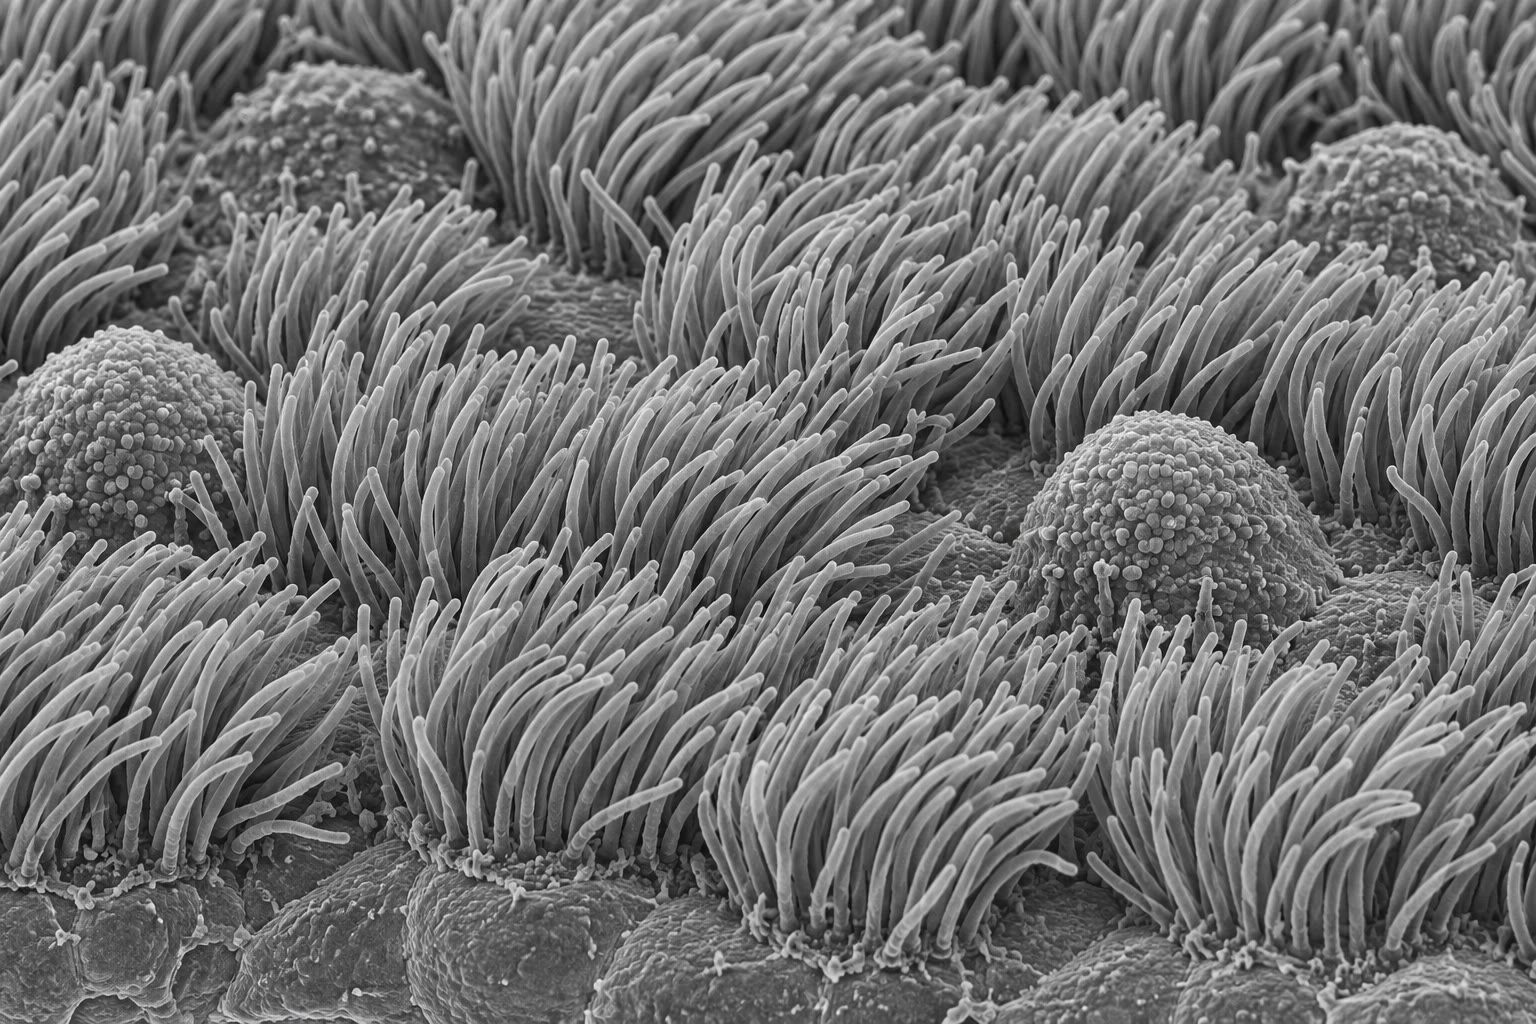
\includegraphics[width=0.54\linewidth]{images/book5/ai/b5-09-cilia-sem.jpg}\hspace{0.03\linewidth}
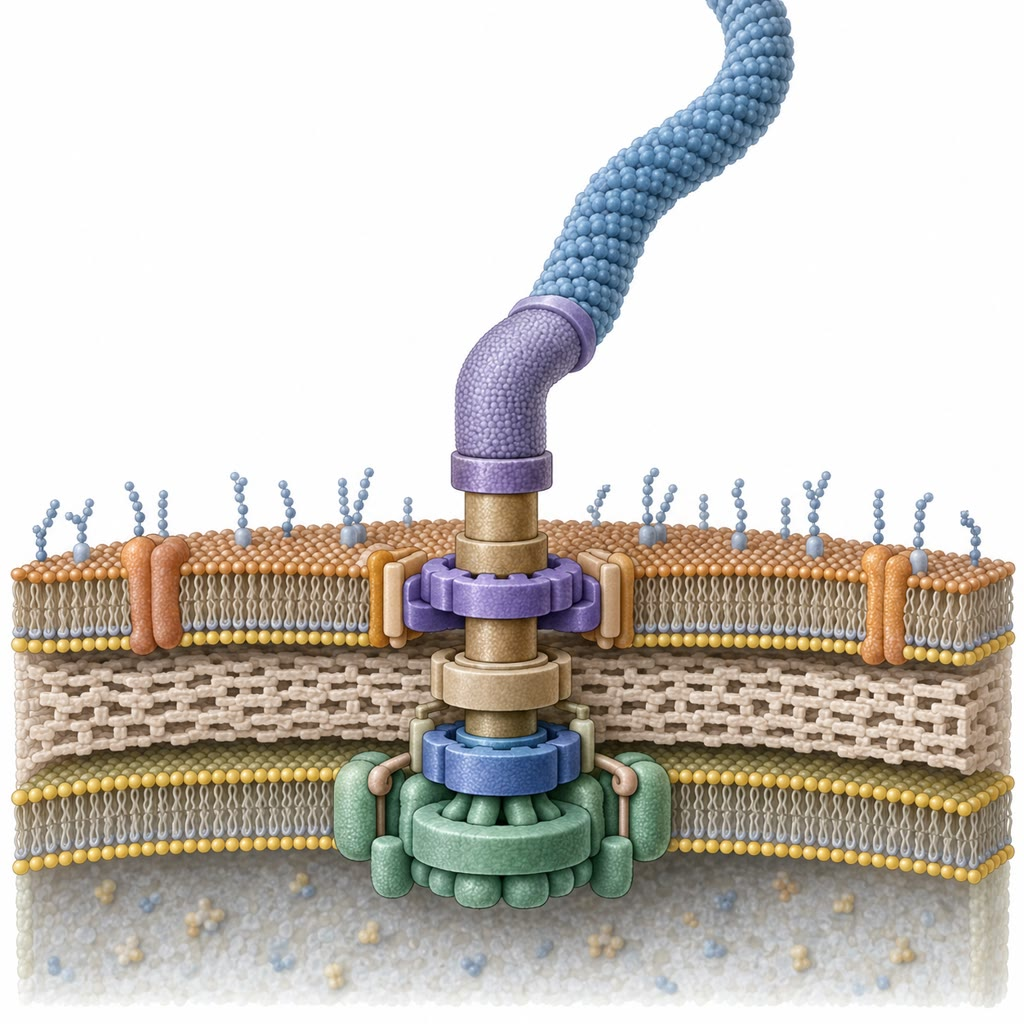
\includegraphics[width=0.36\linewidth]{images/book5/ai/b5-09-flagellar-motor.jpg}

{\small Izquierda: el epitelio ciliado de la tráquea en el microscopio
electrónico de barrido, una pradera de \omterm{def:b3:cytoskeleton-motility:cilia}{cilios} entre células
secretoras de moco con forma de cúpula. Derecha: el \omterm{prop:b3:cytoskeleton-motility:flagellar-motor}{motor flagelar}
bacteriano, una máquina rotatoria de anillos en la envoltura celular
impulsada por el flujo de protones.}
\end{omfigure}

\begin{proposition}[El motor flagelar bacteriano]\label{prop:b3:cytoskeleton-motility:flagellar-motor}
\index{motor flagelar}\index{carrera y voltereta}
El flagelo bacteriano no está emparentado con el eucariota: es un
filamento helicoidal rígido de flagelina, de \qty{20}{nm} de grosor y
varios micrómetros de largo, girado por un \emph{motor rotatorio}
embebido en la envoltura celular --- un rotor de unas cuarenta y cinco
proteínas rodeado por un anillo de unidades estatoras, cada una un canal
por el que los protones fluyen a favor de su gradiente hacia el interior,
unos mil protones por vuelta. El motor gira hasta a \qty{300}{Hz},
invierte el sentido en un milisegundo y desarrolla un par de unos
\qty{1000}{pN.nm}; está construido con unas veinte proteínas cuyos genes
se encienden en el orden en que se ensamblan las piezas, de dentro afuera.
En \emph{E.~coli}, la rotación antihoraria agrupa los varios flagelos en
una hélice propulsora y la célula \emph{corre} en línea recta; un cambio
al sentido horario deshace el haz y la célula da una \emph{voltereta}
hasta una dirección nueva al azar. La vía de la quimiotaxis no sesga nada
más que la frecuencia de volteretas --- menos cuando las condiciones
mejoran --- y eso basta para remontar un gradiente.
\end{proposition}

\begin{remark}[El citoesqueleto es un verbo]\label{rem:b3:cytoskeleton-motility:verb}
Casi nada de lo descrito en este capítulo es una estructura en el sentido
en que lo es un hueso: el \omterm{def:b3:cytoskeleton-motility:migration}{lamelipodio} es una onda de polimerización, el
huso del \cref{ch:b3:cell-cycle-apoptosis} un estado estacionario de
\omterm{def:b3:cytoskeleton-motility:filaments}{microtúbulos} que crecen y se desploman, y el batido del \omterm{def:b3:cytoskeleton-motility:cilia}{cilio} un patrón
de conmutación de motores. El recambio no es un coste que la célula
tolere, sino el mecanismo mismo, que es por lo que todos estos sistemas
funcionan con hidrólisis de nucleótidos y se detienen en cuestión de
minutos cuando falta el ATP, y por lo que los venenos que congelan los
polímeros en cualquiera de los dos estados --- taxol o colchicina,
faloidina o citocalasina --- son igual de letales.
\end{remark}

\section{Ejercicios}

\begin{exercise}[$\star$]\label{exo:b3:cytoskeleton-motility:1}
Compárense los \omterm{def:b3:cytoskeleton-motility:filaments}{filamentos de actina}, los \omterm{def:b3:cytoskeleton-motility:filaments}{microtúbulos} y los \omterm{def:b3:cytoskeleton-motility:filaments}{filamentos
intermedios} en diámetro, subunidad, polaridad, nucleótido y papel típico.
\end{exercise}

\begin{exercise}[$\star$]\label{exo:b3:cytoskeleton-motility:2}
Defínase la \omterm{thm:b3:cytoskeleton-motility:treadmilling}{concentración crítica}. ¿Por qué los dos extremos de un
\omterm{def:b3:cytoskeleton-motility:filaments}{filamento de actina} tienen concentraciones críticas distintas, y qué
ocurriría si fueran iguales?
\end{exercise}

\begin{exercise}[$\star$]\label{exo:b3:cytoskeleton-motility:3}
Nómbrese un motor para cada caso: una vesícula hacia la periferia
celular por \omterm{def:b3:cytoskeleton-motility:filaments}{microtúbulos}; una vesícula hacia el centro; la contracción de
una fibra de tensión; la flexión de un \omterm{def:b3:cytoskeleton-motility:cilia}{cilio}. Dese el sentido que toma
cada uno en su vía.
\end{exercise}

\begin{exercise}[$\star$]\label{exo:b3:cytoskeleton-motility:4}
Enumérense los cuatro pasos del ciclo del reptar y la GTPasa de la
familia Rho que gobierna cada uno de los tres primeros.
\end{exercise}

\begin{exercise}[$\star\star$]\label{exo:b3:cytoskeleton-motility:5}
El extremo más de un polímero tiene
$k_{\text{on}} = \qty{5}{\micro M^{-1}.s^{-1}}$ y
$k_{\text{off}} = \qty{1}{s^{-1}}$, y su extremo menos $k_{\text{on}} =
\qty{1}{\micro M^{-1}.s^{-1}}$, $k_{\text{off}} = \qty{0.8}{s^{-1}}$.
Hállense las dos concentraciones críticas, la concentración estacionaria
y la velocidad de la noria en subunidades por segundo y, para subunidades
de \qty{2.7}{nm}, en nanómetros por segundo.
\end{exercise}

\begin{exercise}[$\star\star$]\label{exo:b3:cytoskeleton-motility:6}
La \omterm{def:b3:cytoskeleton-motility:motors}{cinesina} camina a \qty{800}{nm/s} con pasos de \qty{8}{nm}, un ATP
cada uno. ¿Cuántos ATP por segundo y por motor? El axón de una neurona
mide \qty{1}{m}: ¿cuánto dura el viaje, y cuántos ATP gasta en él un
motor? Compárese con el tiempo de difusión de la
\cref{prop:b3:cytoskeleton-motility:physics}.
\end{exercise}

\begin{exercise}[$\star\star$]\label{exo:b3:cytoskeleton-motility:7}
La \omterm{def:b3:cytoskeleton-motility:motors}{miosina} V da pasos de \qty{36}{nm} por ATP. ¿Cuál es su \omterm{prop:b3:cytoskeleton-motility:physics}{fuerza de
parada} máxima, y por qué es menor que la de la \omterm{def:b3:cytoskeleton-motility:motors}{cinesina}? ¿Qué motor
conviene más para llevar una carga grande, y cuál para moverse deprisa?
\end{exercise}

\begin{exercise}[$\star\star$]\label{exo:b3:cytoskeleton-motility:8}
Predígase el efecto sobre una célula en división, y sobre una célula que
repta, de (a) el taxol, (b) la colchicina, (c) la citocalasina, (d) un
inhibidor de Rac, y explíquese cada uno a partir del mecanismo.
\end{exercise}

\begin{exercise}[$\star\star$]\label{exo:b3:cytoskeleton-motility:9}
En un experimento de FRAP sobre un \omterm{def:b3:cytoskeleton-motility:migration}{lamelipodio}, la fluorescencia se
recupera con un semitiempo de \qty{20}{s} hasta el \qty{90}{\%} de su
valor inicial. ¿Cuáles son el tiempo de permanencia de la actina en la
red y la fracción inmóvil? Las motas fluyen hacia atrás a
\qty{1.5}{\micro m/min} mientras el borde avanza a \qty{1}{\micro m/min}:
¿a qué velocidad polimeriza la actina en el borde?
\end{exercise}

\begin{exercise}[$\star\star\star$]\label{exo:b3:cytoskeleton-motility:10}
Explíquese la \omterm{def:b3:cytoskeleton-motility:instability}{inestabilidad dinámica} en términos de la \omterm{def:b3:cytoskeleton-motility:instability}{caperuza de GTP}, y
muéstrese por qué una población de \omterm{def:b3:cytoskeleton-motility:filaments}{microtúbulos} mantenida justo por
encima de la \omterm{thm:b3:cytoskeleton-motility:treadmilling}{concentración crítica} se vuelve bimodal en longitud en lugar
de uniforme. ¿Qué gana la célula con un comportamiento que malgasta GTP?
\end{exercise}

\begin{exercise}[$\star\star\star$]\label{exo:b3:cytoskeleton-motility:11}
Una bacteria de \qty{2}{\micro m} nada a \qty{25}{\micro m/s}. En agua a
esta escala domina la fricción viscosa y la célula se detiene en un
nanómetro cuando el motor para. Explíquese por qué un movimiento
recíproco (un remo) no puede propulsarla y una hélice que gira sí, y
estímese el número de protones que gasta el motor por segundo a
\qty{100}{Hz}.
\end{exercise}

\begin{exercise}[$\star\star\star$]\label{exo:b3:cytoskeleton-motility:12}
El síndrome de Kartagener --- \omterm{def:b3:cytoskeleton-motility:cilia}{cilios} inmóviles --- da bronquitis
crónica, infertilidad masculina y, en la mitad de los pacientes, el
corazón en el lado derecho. Explíquese cada cosa a partir de la biología
del \omterm{def:b3:cytoskeleton-motility:cilia}{axonema}, y dígase por qué lo último afecta solo a la mitad.
\end{exercise}

\section{Problema: un neutrófilo en marcha}

\begin{problem}[{Problema de fin de semana --- el presupuesto de actina
de un neutrófilo contado, su noria de subunidades calculada, el viaje de
una vesícula por un axón cronometrado frente a la difusión, la eficiencia
de un motor medida y la polimerización y el coste en ATP del frente que
repta resueltos, hasta llegar a la velocidad de la noria, al tiempo para
recorrer un axón y al ATP que quema un lamelipodio por segundo}]
\label{pb:b3:cytoskeleton-motility:1}
Datos: un neutrófilo de \qty{300}{\micro m^3} de volumen contiene actina
a \qty{200}{\micro M}, la mitad polimerizada; una subunidad añade
\qty{2.7}{nm} a un filamento. Constantes de velocidad de la actina como
en \cref{ex:b3:cytoskeleton-motility:actin-numbers}. \omterm{def:b3:cytoskeleton-motility:motors}{Cinesina}: pasos de
\qty{8}{nm}, \qty{800}{nm/s}, \omterm{prop:b3:cytoskeleton-motility:physics}{fuerza de parada} \qty{6}{pN}; hidrólisis
del ATP $\Delta G = \qty{50}{kJ/mol}$; $k_{B}T = \qty{4.1}{pN.nm}$;
coeficiente de difusión de la vesícula \qty{1}{\micro m^2/s}; longitud
del axón \qty{1}{m}. El \omterm{def:b3:cytoskeleton-motility:migration}{lamelipodio} mide \qty{20}{\micro m} de ancho con
$200$ filamentos por micrómetro de borde y avanza a \qty{10}{\micro
m/min}; la red se desensambla \qty{3}{\micro m} por detrás del borde.

\medskip
\noindent\textbf{Parte I --- El presupuesto de actina.}
\begin{enumerate}
  \item ¿Cuántas moléculas de actina contiene la célula, y cuántas están
        en filamentos?
  \item ¿Qué longitud total de filamento es esa? Si el filamento medio
        mide \qty{0.25}{\micro m}, ¿cuántos filamentos hay?
  \item La actina libre está a \qty{100}{\micro M}, muy por encima de la
        \omterm{thm:b3:cytoskeleton-motility:treadmilling}{concentración crítica} del extremo barbado. ¿Por qué no crecen sin
        más los filamentos hasta agotar el monómero? (Dos proteínas.)
  \item La noria in vitro: calcúlense $C_{\text{ss}}$ y $J$ a partir de
        las constantes de velocidad, y la velocidad de la noria en
        nanómetros por segundo y en micrómetros por minuto.
  \item En la célula la velocidad efectiva es \qty{1}{\micro m/min}. ¿Por
        qué factor aceleran los reguladores al polímero desnudo?
  \item Cada subunidad que pasa por la noria cuesta un ATP. Si los
        $2\times 10^{5}$ filamentos funcionaran como norias a la
        velocidad celular, ¿cuántos ATP por segundo, y qué fracción es
        eso del recambio total de una célula, de unos $10^{9}$ ATP por
        segundo?
\end{enumerate}

\medskip
\noindent\textbf{Parte II --- Una vesícula por el axón.}
\begin{enumerate}[resume]
  \item ¿Cuánto tarda una vesícula movida por \omterm{def:b3:cytoskeleton-motility:motors}{cinesina} en recorrer el
        axón, y cuántos pasos y cuántos ATP gasta el motor?
  \item ¿Cuánto tardaría la difusión en \qty{1}{m}? ¿Y en
        \qty{10}{\micro m}, la anchura de un cuerpo celular? ¿Qué dice la
        comparación sobre dónde pueden permitirse las células fiarse de
        la difusión?
  \item Calcúlense la energía por ATP en julios y en unidades de
        $k_{B}T$.
  \item La fuerza máxima de un motor con pasos de \qty{8}{nm}, y la
        eficiencia de la \omterm{def:b3:cytoskeleton-motility:motors}{cinesina} en la parada.
  \item Una vesícula de \qty{100}{nm} de radio en un citoplasma de
        viscosidad \qty{0.01}{Pa.s} (diez veces la del agua) que se mueve
        a \qty{800}{nm/s} sufre una fricción $F = 6\pi\eta r v$.
        Calcúlese, y compárese con la \omterm{prop:b3:cytoskeleton-motility:physics}{fuerza de parada}: ¿cuántos motores
        hacen falta?
  \item El axón de una neurona lleva unas $10^{4}$ vesículas a la vez.
        ¿Cuál es el consumo total de ATP del transporte, por segundo, y
        cómo se compara con el coste de disparo de la neurona, de unos
        $10^{9}$ ATP por segundo? ¿Qué implica esto para una neurona
        cuyas mitocondrias fallan?
\end{enumerate}

\medskip
\noindent\textbf{Parte III --- El frente.}
\begin{enumerate}[resume]
  \item Conviértase la velocidad del borde a nanómetros por segundo y
        calcúlese el número de subunidades por segundo que cada filamento
        ha de añadir para seguir el ritmo.
  \item ¿Cuántos filamentos empujan el borde, y cuántas subunidades por
        segundo consume todo el borde?
  \item Cada subunidad añadida es un ATP hidrolizado y luego reciclado.
        ¿ATP por segundo para la protrusión? ¿Fracción de los $10^{9}$
        por segundo de la célula?
  \item La red situada tras el borde tiene \qty{3}{\micro m} de fondo y
        se desensambla ahí. ¿Cuál es la vida de una subunidad en la red,
        y cuántas subunidades hay en la red en cada instante?
  \item La membrana se resiste a la protrusión con una fuerza de
        alrededor de \qty{1}{pN} por filamento. Calcúlese el trabajo
        realizado por subunidad añadida ($F\times \qty{2.7}{nm}$) en
        unidades de $k_{B}T$ y dígase si el trinquete browniano --- una
        fluctuación térmica que abre un hueco de \qty{2.7}{nm} --- es
        verosímil.
  \item ¿Por qué la cola cometaria de Listeria no necesita motor, y con
        qué rapidez puede empujar si recluta la misma maquinaria?
\end{enumerate}

\medskip
\noindent\textbf{Parte IV --- La dirección.}
\begin{enumerate}[resume]
  \item El neutrófilo detecta un quimioatrayente cuya concentración sube
        un \qty{2}{\%} a lo ancho de sus \qty{10}{\micro m}. Con
        \num{50000} receptores y un $K_{d}$ igual a la concentración
        media, ¿cuántos receptores más están ocupados en la mitad
        delantera que en la trasera? (Ocupación $\theta = C/(C +
        K_{d})$; úsese la mitad de los receptores por lado.)
  \item La fluctuación aleatoria del número de ocupados en un lado es
        aproximadamente la raíz cuadrada de ese número. ¿Es detectable en
        un solo instante la diferencia de la pregunta 19? ¿En qué ayuda
        promediar durante unos segundos?
  \item ¿Qué GTPasa ha de activarse en el frente y cuál en la parte
        trasera para que la célula gire hacia la fuente? ¿Qué haría una
        célula con Rac constitutivamente activa por todas partes?
  \item La célula llega a la bacteria en \qty{3}{min} desde
        \qty{30}{\micro m} de distancia. Compruébese la velocidad frente
        a los datos.
  \item Una célula sin Arp2/3 se mueve en cambio por ampollas --- bultos
        de membrana impulsados por la presión. ¿Qué paso del ciclo se ha
        sustituido, y qué dice eso sobre el papel de la actina en los
        demás pasos?
  \item Todo el ciclo del reptar dura minutos, y sin embargo la célula
        gira en segundos cuando el gradiente se desplaza. Explíquese,
        usando la vida de la red de la pregunta~16.
  \item Resúmase: la velocidad de la noria in vitro (pregunta~4), el
        tiempo que tarda una vesícula en recorrer el axón (pregunta~7) y
        el ATP por segundo gastado en la protrusión (pregunta~15).
\end{enumerate}
\end{problem}
